\documentclass[a4paper,12pt]{article}

\usepackage{isolatin1}
\usepackage{verbatim}
\usepackage{palatino}
\usepackage{color}
\usepackage{xspace}
\usepackage{hyperref}
\usepackage{graphicx}


%%% -- Configuration ----------------------------------------------------

\hyperbaseurl{file://../hdoc/}

%
% Colour setup (to come?)
%

\definecolor{linkcol}{rgb}{0.1,0.1,0.4} % dark blue

\ifx\hypersetup\undefined\relax\else
 \hypersetup{%
    %breaklinks=true,
    colorlinks=true,
    %hyperindex=true,
    pdfpagemode=None,
    linkcolor=linkcol,
    citecolor=linkcol,
    %plainpages=false,
    hypertexnames=false
 }
\fi


%%% -- Useful macros ----------------------------------------------------

%% The code environment typesets its contents verbatim.
\def\code{\verbatim}
\def\endcode{\endverbatim}
%% Same typesetting as code, but different name; this is
%% for code you do not want to show up in literal scripts. 
%% (i.e. the code with syntax errors in it :-)
\def\xcode{\verbatim}
\def\endxcode{\endverbatim}
%% Code snippets in the text:
% \def\codetxt{\textcolor{codecol}\verb} %% hmm...
% \let\MMTextTT=\texttt{}
% \renewcommand{\texttt}[1]{\textcolor{codecol}{\MMTextTT{#1}}}


\title{A Short Introduction to \HTk \\
  Graphical User Interfaces for Haskell Programs}

\author{Christoph L�th \\ FB 3 -- Mathematik und Informatik,
  Universit�t Bremen}

\newcommand{\HTk}{\textsc{HTk}\xspace}

\newcommand{\ToBeDone}[1]{\textbf{TBD: #1}}

\begin{document}

\maketitle{}

\section{Getting Started}

This article is an introduction to the basics of \HTk, a toolkit to
build graphical user interfaces (GUIs) in Haskell. \HTk{} is based on
an encapsulation of Tcl/Tk \cite{Ousterhout,Welch}, but we will not
assume any previous knowledge of Tcl/Tk. The article is meant as a
rough guide and introduction to the structure of HTk; it is not meant
as a complete reference manual. Rather, it should give readers enough
information and background to get them started on their first HTk
programs, to know which parts of HTk might be potentially useful in
the applications they have in mind, what is feasible to build with HTk
and what not, and finally to enable them to find further information
quickly in the \href{index.html}{online reference material}.

\subsection{Basics}

When we design and implement a graphical user interface, we have to
take two aspects into account: the \emph{static} aspect, 
which is to specify its appearance (which buttons to place where, what
menues to display, etc.), and the \emph{dynamic} aspect, which
specifies its behaviour in reaction to the user's actions. 

In \HTk, these two aspects are modelled by \emph{monads}. The dynamic
aspect is modelled in the \texttt{IO} monad, where all of Haskell's
external interactions takes place. The dynamic aspect is modelled by
\emph{events}. For a more complete description of events, we refer to
\cite{ger:Events}. For the time being, events are an abstract datatype
with two main operations.

The central operation is \texttt{sync :: Event a-> IO a} which holds
the current thread until an event of type \texttt{Event a} occurs.
Further, \texttt{(>>>=) :: Event a-> (a-> IO b)-> Event b} takes an
event and an IO action, and returns an event, which when we sync on it
performs the IO action after successful synchronisation. As with the
monad composition, \texttt{(>>>)::Event a-> IO b-> Event b} is the
derived version where the second function throws away its argument.

Moreover, events form a monad, which allows us to build complex
behaviour from basic behaviours in a compositional way by the monad's
composition.

Events are always embedded in the \texttt{IO} monad with the
\texttt{sync} operation. That the dynamic behaviour is not modelled
with \texttt{IO} actions directly reflects the fact that user
interaction in a graphical user interface is different from other
forms of IO, because it happens \emph{asynchronously}.

Further, events allow the user interface to be concurrent in a natural
and controlled way, which allows for a reasonable degree of
concurrency which is still tractable.

\input{Mainsimple1.lhs}

\input{Mainsimple2.lhs}

\subsection{Structure of this Paper}

The rest of this short paper is organized as follows: we will first
explain the organization of the datatypes modelling the static
behaviour of the graphical user interface. In
section~\ref{sec:events}, we will describe events and in particular
how to generate them from user input. After this, we will describe
every widget in detail.


\section{Elements of \HTk}

In general, \HTk has a couple of abstract datatypes used to model
elements of the graphical user interface, such as buttons, menues,
short text fields, longer text fields and so on. Let us examine the
buttons used in Section~\ref{ssec:ex1} above. There is an abstract
datatype \texttt{Button}, created with the following function
\begin{xcode}
newButton :: Container par=> par-> [Config Button]-> IO Button
\end{xcode}

Let us first examine the class \texttt{Container}. 

\subsection{The GUI element hierarchy and the \texttt{Container} class.}

The class \href{Packer.html#Container}{\texttt{Container}} designates
GUI elements into which other GUI elements may be packed.

Instances of \texttt{Container} include \texttt{Toplevel} (windows),
\texttt{HTk} (Tk's root window), and \texttt{Frame}; furthermore
\texttt{Canvas}, and and \texttt{Editor} (and a few Tix widgets).

The class \texttt{Container} is \emph{abstract} --- it has no class
functions, and only serves to structure the code. Abstract classes are
used frequently in HTk to impose a typing discipline onto Tk's untyped
GUI element structure, with the benefit that type checking can prevent
run time errors.


\subsection{Configurations and Resources}

Above, the text of the button was set with a \emph{configuration
  option}. Configuration options determine various attributes of a
widget. They can be given at the time of creation, or changed later
on. Not every widget supports all configurations, and this behaviour
is modelled in HTk by Haskell's type classes: configurations in
general are polymorphic over all widgets, but particular
configurations are restricted to certain classes of widgets.

For example, the text configuration is given by this class:
\begin{xcode}
class (GUIObject w, GUIValue v) => HasText w v where
  text :: HasText w v => v -> Config w
  getText :: HasText w v => w -> IO v
\end{xcode}
The class \texttt{GUIObject w} is one of HTk's most basic classes. Its
instances are widgets, and other interface elements we will encounter
later (canvas items, text tags). \texttt{GUIValue v} is another basic
class, the instances of which are all basic datatypes which can be
communicated to Tk: \texttt{Int}, \texttt{Double}, \texttt{Bool},
\texttt{String} and \texttt{[String]}. 

Widgets can be configured with a text are instances of the class
\texttt{HasText}, such as \texttt{Button}. 

The configuration classes can all be found in the module
\href{Configuration.html}{\texttt{Configuration}}.

The configuration type is just a type synonym\footnote{Type synonyms
  like that in class confusions confuse Hdoc, which is why they appear
  expanded at various places of HTk's source code--- just in case you
  happen to browse it, which you are more than welcome to.}
\begin{xcode}
type Config w = w -> IO w
\end{xcode}
As seen above, configurations can be given at the time of creation, or
later on. In the latter case, the helpful \texttt{(\#)} operator
provides useful syntactic sugar:
\begin{xcode}
( # ) :: a -> (a -> b) -> b
o # f = f o  
\end{xcode}

Note the difference between configuration options, which determine the
appearance, and behaviour of the widget, and packing options, which
determine the way it is packed. 

\subsubsection{Geometry}

The abstract data type \texttt{Distance}, implemented in the module
\href{Geometry.html}{\texttt{Geometry}}, represents distances in HTk.
Distances can be specified in \texttt{cm}, \texttt{mm}, \texttt{ic}
(inches) and \texttt{pp} (points), with functions  \texttt{cm:: Int->
  Distance}. Moreover, \texttt{Distance} is an instance of
\texttt{Num}, so we can specify the distance 3 (meaning 3 pixels)
directly. 

\subsubsection{Colours}

The abstract data type \texttt{Colour}, implemented in the module
\href{Geometry.html}{\texttt{Geometry}}, represents colours in
HTk. Just like distances, the type itself is abstract, but unlike
distances, there is a class \texttt{ColourDesignator}, the instances
of which give ways of describing colours, such as:
\begin{xcode}
instance ColourDesignator [Char]
instance ColourDesignator (Int, Int, Int)
instance ColourDesignator (Double, Double, Double)  
\end{xcode}
The strings are named colours (\texttt{red}, \texttt{white},
\texttt{black}, etc.), the tuples are RGB values. (The functions of
the type classes \texttt{Colour} and \texttt{ColourDesignator} are for
HTk's internal consumption only.)

\subsubsection{Fonts}

Fonts are implemented in the module
\href{Font.html}{\texttt{Font}}. They are specified in the usual way,
by giving a family, slant, spacing, width and weight. For example, the
family is given by 
\begin{xcode}
data FontFamily = Lucida | Times | Helvetica 
                | Courier | Symbol | Other String  
\end{xcode}
where the five enumerated types are available on most systems. With
\texttt{Other}, you can directly give a more exotic family such as
\texttt{clearlyu alternate glyphs}. 

Be warned that fonts are, in principle, not very portable under X,
since the available fonts are determined by the fonts of the X server
the programm is running on. It is best to stick to well-known font
families such as the above, and usual sizes. 

\subsection{Packing}

As mentioned above, after widgets have been created (with e.g.
\texttt{newButton}), they will not be displayed yet; this only happens
after they have been packed. One can use this effect by first creating
lots of widgets, and then packing them in one go, lessening the
unpleasant flicker effect occuring when the GUI is built one interface
at a time.\footnote{Unfortunately, this effect cannot be totally
  eliminated.}

Packing in particular determines the visual layout of the GUI by the
order in which the widgets are packed, and by packing options. Tk's
know different packing algorithms (or \emph{geometry managers}, in Tk
parlance); of these, HTk supports the standard packer, and the grid
packer.


\subsubsection{The Standard Packer}

The behaviour of the standard packer is easily explained, and hard to
understand. Widgets are packed with the function
\begin{xcode}
pack::Widget w => w -> [PackOption] -> IO ()  
\end{xcode}

The datatype
\href{PackOptions.html#PackOptions.PackOption}{PackOption}
is defined as 
\begin{xcode}
  data PackOption = Side SideSpec  | Fill FillSpec 
                  | Expand Toggle  | Anchor Anchor
                  | IPadX Distance | IPadY Distance
                  | PadX Distance  | PadY Distance
\end{xcode}
The first two constructors are most important here. The
\href{PackOptions.html#PackOptions.SideSpec}{SideSpec}
specifies where the widget is packed (top, bottom, left, right)e, and
\href{PackOptions.html#PackOptions.FillSpec}{FillSpec}
specifies in which direction it expands to fill the available space.
Bear in mind that widgets are packed as tight as possible (in
particular into windows), and that once packed, they are never
repacked. That is, if e.g. a widget is packed against the top, it will
sit in the middle (if no \texttt{Fill X} is specified), and will not
move if a widget is packed against the right-hand side.

\texttt{Expand} just means that the widget expands when the containing
element is expanded (i.e. the window is resized), and \texttt{Anchor}
specifies a gravity (a side to which the widgets stick). The rest
create a padding border around the widget in various directions.

It is quite normal that most of the times the packing will not look
like intended, and you will need to use frame widgets (see
\ref{ssec:frames}).

\subsubsection{The Grid Packer}

The grid packer divides the container widget into a grid, and allows
placement of widgets relative to that grid. To pack a single widget
use the 
\href{Packer.html#Packer.grid}
{following function:}
\begin{xcode}
grid :: Widget w => w -> [GridPackOption] -> IO ()
\end{xcode}

The datatype
\href{GridPackOptions.html#GridPackOptions.GridPackOption}
{\texttt{GridPackOptions}} specifies the packing options for the grid
packer.

Note that within the same container you cannot use different packing
algorithms. The first widget packed into a container defines the
packing for this container.

\section{Events}

In general, events are an abstract datatype for communication and
synchronisation, much in the spirit of process algebras such as CCS
\cite{Milner:CommunicationConcurrency}, CSP \cite{Hoare,Roscoe} or
the $\pi$ calculus \cite{Milner:PiCalculus}. Here, an 
\href{Events.html}{\texttt{Event}} is
an abstract datatype with operations such as \texttt{sync},
\texttt{+>} and \texttt{>>>=}, which additionally form a monad; we
refer to \cite{ger:Events} for more information. 

In \HTk, events are mostly generated from user interactions by means
of the \emph{bind} commands. By binding a user interaction (such as
clicking a button), we set it up to produce an event, on which we can
synchronise and thus produce a reaction to the user's action.

One important caveat here is that once you set up a binding, you
\emph{must} eventually synchronise on the resulting events, since
otherwise the unused events will pile up and result in a memory leak.

Bindings are generated by calling one of \texttt{clicked},
\texttt{bindSimple} and \texttt{bind}, where \texttt{bind} is most
flexible, which shows up in the type.

\subsection{Simple Clicks}
Simple interface elements such as buttons and menu entries which
  are instances of the class
  \href{HTk.html#HTk.HasCommand}{\texttt{HasCommand}}. For these, we
  have a function
\begin{xcode}    
clicked :: HasCommand w => w -> IO (Event ())
\end{xcode} 
  The event here occurs when the element is clicked. The event does
  not have any additional information. 

\subsection{Simple Binds}
For all GUI elements, the function
  \href{HTk.html#HTk.bindSimple}{\texttt{bindSimple}} 
\begin{xcode}    
bindSimple::GUIObject wid => wid -> WishEventType -> IO (Event (), IO ())
\end{xcode}
where \href{HTk.html#HTk.WishEventType}{\texttt{WishEventType}} is an
algebraic data type describing the kind of event we would like to bind
to, much along the lines of Tk's events which in turn are given by X
events. Each constructor corresponds to a different event, such as
\begin{itemize}
\item mouse buttons pressed and released (\texttt{ButtonPress (Maybe
    Int)}, \texttt{ButtonRelease (Maybe Int)}),
\item mouse movements (\texttt{Motion}),
\item the mouse entering or leaving a GUI element (\texttt{Enter},
  \texttt{Leave}),
\item keys pressed or release (\texttt{KeyPress (Maybe KeySym)},
  \texttt{KeyRelease (Maybe KeySym)}),
\item and various window events (\texttt{Map}, \texttt{Unmap},
  \texttt{Expose}, \ldots).
\end{itemize}
Note that not every GUI element can generate every event. Obviously,
only windows can generate window events, but more subtly, only entry
widgets, editor widgets and windows can generate \texttt{Key} events.

The return value of \texttt{bind} is an event, and an IO action which
unbinds the event. You should use this action if you are not
interested in the event anymore (i.e. it will not be synchronised on
anymore), otherwise there will be a memory leak.

\subsection{Full Bindings}

In fact, \texttt{bind} is only a simplified version of the
  function \href{HTk.html#HTk.bind}{\texttt{bind}}
\begin{xcode}
bind::GUIObject wid => wid -> [WishEvent] 
                       -> IO (Event EventInfo, IO ())
data WishEvent = WishEvent [WishEventModifier] 
                           WishEventType
\end{xcode}
where
\href{HTk.html#HTk.WishEventModifier}{\texttt{WishEventModifier}}
desribes possible event modifiers such as \texttt{Shift},
\texttt{Alt}, \texttt{Meta} (corresponding to the Shift, Alt or Meta
key being held), \texttt{Button1}, \ldots, \texttt{Button5}
(corresponding to mouse button 1 thru 5 being pressed) or \texttt{Double} and
\texttt{Triple}. Again, not all combinations of modifiers and events
make sense; for example, double and triple pertain to mouse button
presses, and modifying a mouse button press with a different button is
not really helpful. Note that the argument of bind is a list of
events, meaning of course that each of the events generates in event
(not only their combination).

Here, the first component of the return value is an event of
\texttt{EventInfo}, which is a labelled record as
follows:\footnote{Unfortunately, HDoc chokes on the relevant part of
  the source right now, so this is not in the reference manual.}
\begin{xcode}
data EventInfo = EventInfo { x :: Distance,
                             y :: Distance,
                             xRoot :: Distance,
                             yRoot :: Distance,
                             button :: Int  
\end{xcode}
The information here is the x and y component of the mouse position,
both relative to the window in which the event occurs, and the root
window (i.e. the screen), and the button being pressed. 

\section{Widgets}

In the following, we give a brief tour around HTk's widgets. These are
essentially Tk's widgets. We have simple widgets which are explained
in short sentences of words with less than three syllables, menues,
text widgets, and canvasses, which require a sllightly longer
explanation. 

There are more widgets: if you can use Tix (you should anyway, it
looks slightly less clunky than plain Tcl/Tk), there are the useful
tab and pane widgets. And because HTk is an abstraction on top of Tk,
there are a variety of so-called \emph{mega-widgets} which are
implemented in Haskell; these can be found in the toolkit
(Sect.~\ref{sec:toolkit}).

\subsection{Basic Widgets}

\begin{itemize}
  
\item Frames

\label{ssec:frames}

A \href{Frame.html}{frame} is just an invisible container into which
we can pack other widgets, grouping them together. The use of frames
is in packing: the grouping is necessary most of the time to achieve
the desired layout with the standard packer.

Moreover, when using a frame, we can use a different packer (see
Sect.~\ref{sec:packing}) than in the parent widget; for example, we
can use the grid packer inside a window using the standard packer.

\item Boxes
  
  \href{Box.html}{Boxes} are mega-widgets, implemented using frames.
  They allow simple horizontal or vertical packing (widgets are placed
  in the box side by side or on top of each other), and be flexible or
  rigid (expand when the parent window is resized, or not); e.g.
  \texttt{newVBox} creates a rigid box with vertical packing, and
  \texttt{newHFBox} creates a flexible box with horizontal packing.

\item Buttons

  A \href{Button.html}{button} is a simple widget which can be
  clicked. Buttons can have bitmaps, images (class \texttt{HasPhoto}),
  or text as labels. 

\item Labels and Messages

  A \href{Label.html}{label} is a simple widget for text, bitmaps or
  images. \href{Message.html}{Messages} are slightly more
  sophisticated widgets for longer text messages; messages line-break 
  the text. For both, the font of the text (class
  \texttt{HasFont}) and the justification (class
  \texttt{HasJustified}) can be specified. 

\input{Mainlist.lhs} %% Scrollbars, List boxes.

\end{itemize}

\input{Mainmenu.lhs} %% Menues 

\subsection{The Textwidget}

\subsection{The Canvas Widget}

\section{The Toolkit}

\label{sec:toolkit}

\section{Larger Examples}

\section{The hsMines Game}

As an example for more complex GUI programming, we will now develop a
GUI for a minesweeper like game called hsMines. Just in case you do
not know Minesweeper or some of its many clones I'll give a short
overview.

\subsection{What's that game?}
Playing Minesweeper you have a grid of about 20x20 similar
fields. Below any of this fields could be a mine or just an empty
field -- you wont know until you click at the field and are eventually
shred to pieces by some nasty mine. Goal of the game is to find all
the mines an mark them with tiny flags. An nearly impossible task. To
make the game any fun you are told the exact amount of mines around
the field you just opened. If this number is 0, it's safe to explore
all the adjacent fields. And because this is a stupid task the
machine does it for you. If you manage to explore all empty fields you
win, if you find one of the mines, you lost, best time gets the
highscore. Simple as that.

For this is not a course in haskell programming I will not spent any
words on the games code itself and will come straight to the very
heart of this section, the hsMines GUI.


\subsection{In the beginning\dots}
\dots, as you should have read, is the window. And for we are running
compiled code here, it's created in the \texttt{main} function.
\begin{code}
main = 
 do htk<- initHTk [withdrawMainWin]
    run htk normalSize 

run :: HTk-> (Int, Int)-> IO ()
run htk currentSize = 
 do main <- createToplevel [text "hsMines"]

finishHTk
\end{code}

Having only this, the GUI would look rather boring, but it's not bad
for just a few lines of code, isn't it? It looks a bit bent in a loop
but we will see later that this is needed to make the field
resizeable.\\
The last line is necessary to clean up all the events we've kicked
loose so far.

\begin{figure}[h]
\begin{center}
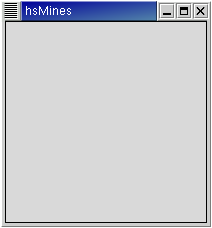
\includegraphics[scale=0.6]{img/Screenshot01}
\caption{The hsMines window}
\end{center}
\end{figure}

\subsection{Menus}

What would a GUI be without them? Somewhat empty as it seems. So let's
create some menus.

\begin{code}
    menubar <- createMenu main False []
    main # menu menubar

    fm <- createPulldownMenu menubar [text "File"]

    restb <- createMenuCommand fm [text "Restart"]
    qutib <- createMenuCommand fm [text "Quit"]

    pm <- createPulldownMenu menubar [text "Preferences"]
   
    pmc1 <- createMenuCascade pm [text "Size"]
    pmc1m <- createMenu main False []
    pmc1 # menu pmc1m
        
    pmc2 <- createMenuCascade pm [text "Difficulty"]
    pmc2m <- createMenu main False []
    pmc2 # menu pmc2m
\end{code}

To this point we create a number of menus and pulldowns. Let's go
through this step by step.
In line 1 we create an menu inside \emph{main} (our window) that was
created in \texttt{run}. In line 2 we tell \HTk to asign this new menu
we call \emph{menubar} to be the menu of \emph{main}.\\
In line 3 (we will not count the empty lines), we create our first
pulldown menu -- that is what actually is normaly called a menu. This
pulldown menu is created inside \emph{menubar}, is called \emph{fm}
and has the charming text "`File"'. For not leaving this menu (or
pulldown menu) empty, we create menu entrys so called menu commands
inside \emph{fm}. So by now we have \emph{restb} and \emph{quitb}
inside \emph{fm} inside \emph{menubar} inside \emph{main}.\\
This is quit nice but we will try to put some more functionality into
our menu besides restarting and quiting the game. And as we read
above, the game grid will be resizeable so we will need another menu
to have these commands in.\\
We create a second pulldown menu in \emph{menubar} called
\emph{pm}. In this menu we nest to submenus called menu
cascades. Each of the cascades has a name, \emph{pmc1} and
\emph{pmc2}, and a String set to it's text. The next step is a bit
tricky. One would expect now to fill the cascades directly with some
commands. But the menu cascades are only containers fit to hold a
menu. So we have to create another two menus inside main and asign
them to the two cascades. These two menus are called \emph{pmc1m} and
\emph{pmc2m} which should be an abreviation "`Prefernce Menu Cascade
1's Menu"' respectivly 2.\\
By now we have a menu which holds two pulldown menus. The
first contains two commands, the second contains two cascades which in
turn each contain a menu again. To make sense of these menus we have
to fill them of course. And finally we have to put some functions
behind those commands and what so ever or this would all be for
naught.

\begin{code}
    varSize <- createTkVariable currentSize
    sr1 <- createMenuRadioButton pmc1m [text "tiny (6x6)", value tinySize,
                                        variable varSize]
    sr2 <- createMenuRadioButton pmc1m [text "small (10x10)", value weeSize,
                                        variable varSize]
    sr3 <- createMenuRadioButton pmc1m [text "normal (15x15)", value normalSize,
                                        variable varSize]
    sr4 <- createMenuRadioButton pmc1m [text "large (20x20)", value bigSize,
                                        variable varSize]
    sr5 <- createMenuRadioButton pmc1m [text "huge (25x25)", value hugeSize,
                                        variable varSize]

    varDiff <- createTkVariable (6:: Int)
    dr1 <- createMenuRadioButton pmc2m [text "easy", value (8::Int),
                                        variable varDiff]
    dr2 <- createMenuRadioButton pmc2m [text "normal", value (6::Int),
                                        variable varDiff]
    dr3 <- createMenuRadioButton pmc2m [text "hard", value (4::Int),
                                        variable varDiff]
    dr4 <- createMenuRadioButton pmc2m [text "nuts", value (3::Int),
                                        variable varDiff]
\end{code}
In the code above we do several new things. First we create a new Tk
variable named \emph{varSize} and a few lines later one called
\emph{varDiff}. These are necessary to remember things we do to our
GUI like in this case switching a button.
Our next step is to create a menu radio button\footnote{
  A radio button is a button with several instances. Each of the
  instances is shown, can be selected and is bound to a different value
  but to the same variable. By selecting one of the instances the
  according value is asign to the variable. Because a variable can
  only have one value at a given time, only one of the instances can
  be selected.}
in each of the two submenus. The first radio button asigns tuples of
Int to the Variable \emph{varSize}, the actual values are given in a
couple of functions above in the code which can be fully seen in the
appendix.
% Hier beachten! Code muss in Appendix!
% Evtl. k�nnen die Funktionen auch wieder gel�scht und hier die
% konkreten Zahlen eingesetzt werden. Eigentlich m�ssten andernfalls
% die anderen Zahlen (f�r die Schwierigkeit) auch in Funktionen
% ausgelagert werden. So ist das inkonsequent.
As you we can see in the code above (in \texttt{main} and
\texttt{run}), currentSize holds the value of normalSize and so by
default the radio button is set to normalSize. Nearly the same happens
to \emph{varDiff} and it's radiobutton just without the hiding
functions.\\
The values of varDiff have to be explicitly casted because by default
TkVariables contain Strings. But still nothing happens besides setting
two varaibles.

\begin{code}
    restartClick <- clicked restb
    quitClick <- clicked quitb

    csr1 <- clicked sr1
    csr2 <- clicked sr2
    csr3 <- clicked sr3
    csr4 <- clicked sr4
    csr5 <- clicked sr5

\end{code}

This rather cryptic peace of codes allows us to bind the commands and
the size radio button(s) to a couple of events. These will occure now
whenever one of the buttons is selected -- "`clicked"'.

\begin{figure}[h]
\begin{center}
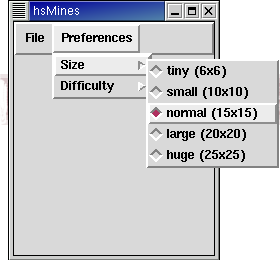
\includegraphics[scale=0.6]{img/Screenshot02}
\caption{The hsMines main window with an open Prefs/Size menu}
\end{center}
\end{figure}

\subsection{The field}

To make all the decoration perfect, wie need the little smiley atop
the playfield which can be used to restart the game.
\begin{code}
    sm <- newButton main [text ":-)"]
    restart2Click <- clicked sm

    pack sm [Side AtTop, PadY 20, PadX 20, Anchor North] 
\end{code}
So we create a Button called sm (from \textbf{sm}iley btw) and bind it
to another Event. And because the GUI does not automaticaly know where
and when to place the button we have to tell it to \texttt{pack sm at
  the top of the main window, pad it 20 pixels wide in any direction
  and keep it align to the upperside} (which is North on most maps).

% \begin{figure}[h]
% \begin{center}
% 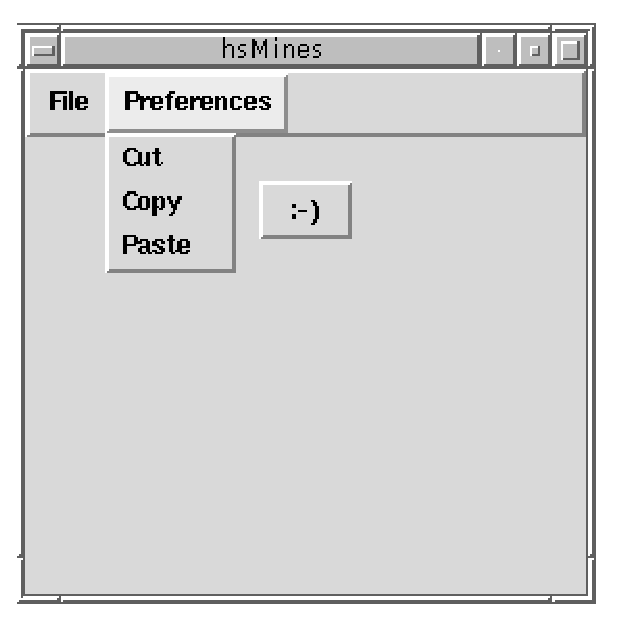
\includegraphics[scale=0.6]{Screenshot3}
% \caption{The hsMines main window with smiley}
% \end{center}
% \end{figure}

I also opened the second menu so you could see Huey, Dewey and
Louie\dots

\begin{code}
    restartCh <- newChannel

    let size= (20, 20)

    bfr <- newFrame main [width (cm 10)]
    allbuttons <- buttons bfr sm (receive restartCh) size 

    pack sm [Side AtTop, PadY 20, PadX 20, Anchor North]

    pack bfr [Side AtTop, PadX 15] 
    mapM_ (\(xy, b)-> grid b [GridPos xy]) allbuttons
    
    -- start the menu handler
    spawnEvent (forever (restartClick >>> sendIO restartCh ()
                      +> restart2Click >>> sendIO restartCh ()
                      +> quitClick >>> destroy main))

\end{code}
To get it realy started we create an IO-channel named restartCh. Then
we create a new Frame (a container widget) with a fixed width and do
somethin strange about allbuttons. Of course this is not that strange.
A function (buttons) is called with some complex arguments and the
result is asigned to allbuttons. We will cover this just some lines
later.

The Frame is packed below the smiley button. They both are told to be
at the top of main, but because only one of them can be there they're
placed below each other in packing order.

To have something to happen with the buttons an Event is spawned. This
single Event listens to some GUI Events we bound some of our buttons
to. Whenever (the Events last until the destruction of the main
thread) one of these three Events occurs, a function is called. The
smiley button and the restart command in the File menu both send an IO
command via the initialised IO channel, the quit command initiates the
destruction of the window and thereby the main thread. If this
happens, finishHTk at the end of the source is reached and the garbage
collection can free all used RAM. But if we don't press one of the
restart buttons, nothing will happen with the many buttons we created
and they all just show a question mark.

% \begin{figure}[h]
% \begin{center}
% \includegraphics[scale=0.2]{Screenshot4}
% \caption{The uninitialised playfield of hsMines}
% \end{center}
% \end{figure}

So all that is left to do in the main function is to initiate the game
for the first time.

\begin{code}
    sendIO restartCh ()
\end{code}

That's all so far. But as you allready know, something happens to
allbuttons in between.

\subsection{The buttons function}

This function has a rather complex signature.

\begin{code}
buttons :: Container par=> par-> Button-> Event() -> (Int, Int)
                           -> IO [((Int, Int), Button)]

\end{code}

For comparison lets have another look on how it's called:

\begin{code}
    allbuttons <- buttons bfr sm (receive restartCh) size   
\end{code}

We have a class restriction on the first argument, par, which has to
be a container. par happens to be just that, a Frame. Lucky us. The
next argument has to be a button as we can happily admit our smiley
buttons is. The third argument has to be an Event. This Event occurs,
when some IO() is send via the IO Channel restartCh and is received by
receive. The last argument is a 2-tuple of Int which is the size of
the game field. Because size is a function with no arguments (thereby
it's a constant value), the field's size can not be changed.

%An dieser Stelle k�nnte man doch eigentlich wunderbar das Menu
%Preferences ins Spiel bringen und eine Reihe von Auswahlgr��en (aka
%Schwierigkeitsleveln) einbauen, oder?

When buttons has done it's work, it will return an IO of a list auf
tuples of tuples of Int an a Button. As you see it is simpler to watch
the signature yourself than to try to puzzle out what I just told you.

The code of buttons is simple a start.


\subsubsection{Create an array of buttons,\dots}

\begin{code}
buttons par sb startEv (size@(xmax, ymax)) =
  do buttons <- mapM (\xy-> do b<- newButton par [text "?"]
                               return (xy, b)) [(x, y) | x <- [1.. xmax],
                                                         y <- [1.. ymax]]
\end{code}

This code is executed no matter what startEv might be! It creates all
the buttons and writes a quotationmark inside so the playfield looks
the way the Figure above shows it.%Verweis auf Figure?
But there is more to happen in the buttons function!


\subsubsection{bind them\dots}

\begin{code}
     let bArr = array ((1,1), size) buttons
         getButtonClick b n xy = 
            do (click, _) <- bindSimple b (ButtonPress (Just (BNo n)))
               return (click >> return xy)
     leCl <- mapM (\(xy, b)-> getButtonClick b 1 xy) buttons
     riCl <- mapM (\(xy, b)-> getButtonClick b 3 xy) buttons
\end{code}

This looks rather complicated but does nothing more than what we did,
when we bound the smiley button to the restart2Click Event. It's just
that we bind the whole Array of buttons we created via a slightly
adjusted Event (\texttt{getButtonClick b 1/3 xy})\footnote{
  As you could surely guess, 2 would be the modifier to get the center
  button bound.
} to two Events.


\subsubsection{and start\dots}

\begin{code}
     spawnEvent start
     return buttons
\end{code}

At the end, we spawn an Event called start and wait. But wait what
for? As you remember an Event is handed over to buttons. And this
event is used to get the game finaly running.

\begin{code}
         start :: Event ()
         start = startEv >>> do m <- createMines (snd (bounds bArr))
                                mapM_ (text " ") (elems bArr)
                                sb # (text ":-)")
                                sync (play m)
\end{code}

This says: If the Event start occurs (by being spawner for example)
and if startEv is the same kind of Event as start (and occurs at the
same time, that is), we execute some more code. Have a look on how we
create mines later, it's of no importance for the GUI. We map over all
elements in the button array and write `` '' to their text. Then we
asign a new smiley to the text of sb (mapM\_ does the same to all the
buttons) and synchronize the start Event to the play Event. No new
Event is created, start just changed into play.

\subsubsection{to play\dots}

\begin{code}
         play :: Mines-> Event ()
         play m = do r <- choose leCl >>>= open bArr m
                     case r of Nothing -> always gameLost >> gameOver
                               Just nu -> play nu
                  +>
                  do r<- choose riCl >>>= flag bArr m
                     play r
                  +>
                  start 
\end{code}

Playing is easy. To play with a set m of mines means to execute three
steps over and over again.

\begin{enumerate}
\item If the left mousebutton is pressed, execute open with the
  button array and the mines. If nothing is left, you loose. If there
  are mines left, you play on.
\item If the right mousebutton is pressed, execute glag with the
  button array and the mines. No evil may occur, just play on.
\item If thing go awry, goto start and wait for the startEv Event.
\end{enumerate}


\subsubsection{until it's over.}

gameLost is just an alert Window to open, to tell you that you've
lost that also changes your smiley into a freak. You are allowed to
kill the messenger.

\begin{code}
         gameLost :: IO ()
         gameLost = do createAlertWin "*** BOOM!***\nYou lost." []
                       sb # (text "X-(")
                       done
\end{code}

Only after you finished up the messenger, the game is realy over, the
\verb�>>� operator takes care of that.

\begin{code}
         gameOver :: Event ()
         gameOver = start 
                    +> 
                    (choose (leCl++ riCl) >> gameOver) 
\end{code}

gameOver is the Event to take over. It leads you back to the start
event, waiting for the startEv Event to occur. If any of the ingame
Events occur, because some dumbhead did not understand the "`BOOM! You
lost."' message or what so ever, the game is still over and nothing
changes.

That's it, anything else is just plain haskell. Naugh, you're right,
there is some tiny tidbits left. Nobody explained how the numbers show
up when an non mine field is explored, right? Okay, we'll come to that
now.

\subsection{Fuzzing around on the play field}




%%% Local Variables: 
%%% mode: latex
%%% TeX-master: "intro"
%%% End: 





\bibliography{intro}
\bibliographystyle{plain}


\end{document}

%%% Local Variables: 
%%% mode: latex
%%% TeX-master: t
%%% End: 
